\begin{frame}
    \frametitle{Problemstellung}
    \begin{itemize}
        \item Sei $\tilde{\phi}(t)$ eine reguläre Funktion die die Spektraldichte schätzt
        \item Alle Annäherungen stetige Funktionen
        \item $\phi(t)$ keine Funktion im eigentlichen Sinne
        \item $\left|\left|\phi(t) - \tilde{\phi}(t)\right|\right|_{L^p}$ nicht definiert
        \item Zwei Möglichkeiten, dies zu umgehen
    \end{itemize}
\end{frame}

\begin{frame}
    \frametitle{Schwartz-Raum über $\R$}
    $$\SR(\R) := \left\{f \in \Cinfty(\R) \mid \forall p, k \in \N_0: \sup_{x \in \R} \left| x^pf^{(k)}(x)\right| < \infty \right\}$$
\end{frame}

\begin{frame}
    \frametitle{Erste Methode}
    Wir benutzen die Tatsache, dass $\delta(t)$ eine Distribution ist:\\
    Sei $g \in \Cinfty(\R)$ eine Testfunktion aus dem Schwartz-Raum $\SR$, dann
    $$\langle \delta(\cdot - \lambda), g \rangle \equiv \int\limits_{-\infty}^{\infty} \delta(t - \lambda) g(t) \dt \equiv g(\lambda)$$
    und für alle $p, k \in \N_0$
    $$\sup_{t \in \R} |t^pg^{(k)}(t)| < \infty$$
    Dann wird der Fehler wie folgt gemessen:
    $$\epsilon_1 = \sup_{g \in \SR} \left| \langle \phi, g \rangle - \langle \tilde{\phi}, g \rangle \right|$$
\end{frame}

\begin{frame}
    \frametitle{Zweite Methode}
    \begin{itemize}
        \item "Regularisierung" der $\delta$-Distribution\\
        \item Ersetzen durch stetige und glatte Funktionen\\
        \item Z.B. Gaussche Normalverteilung mit angemessener Standardabweichung $\sigma$\\
        \item Diese Funktion $\phi_{\sigma}(t)$ ist dann wohldefiniert\\
        \item Berechne Fehler für $p=1, 2$ und $\infty$:
    \end{itemize}
    \vspace{3mm}
    $$\epsilon_2 = \left|\left| \phi_{\sigma}(t) - \tilde{\phi}(t) \right|\right|_p$$
    \vspace{7mm}
    Diese beiden Methoden sind eng verwandt!
\end{frame}

\begin{frame}
    \frametitle{Der Begriff der Auflösung}
    \begin{itemize}
        \item Selten Bedarf für exakte Annäherung aller Eigenwerte von $A$
        \item Oft nur Eigenwerte in $[a, b] \subset \sigma(A)$
        \item $b - a$ heißt \emph{Auflösung} der Schätzung
        \item Je kleiner das $\sigma$ in $\epsilon_2 = \left|\left| \phi_{\sigma}(t) - \tilde{\phi}(t) \right|\right|_p$, desto höher die Auflösung
        \item Für $\epsilon_1 = \sup_{g \in \SR} \left| \langle \phi, g \rangle - \langle \tilde{\phi}, g \rangle \right|$ reguliert man über die Testfunktionen
    \end{itemize}
\end{frame}

\begin{frame}
    \frametitle{Noch mehr Probleme mit Dirac}
    Betrachte
    $$\nu_{[a, b]} = \int\limits_a^b n \phi(t) \dt$$
    Definiere entsprechend
    $$\tilde{\nu}_{[a, b]} = \int\limits_a^b n \tilde{\phi(t)} \dt$$
    mit $\tilde{\phi}(t) \in \Cinfty(\R)$
\end{frame}

\begin{frame}
    \frametitle{Noch mehr Probleme mit Dirac (2)}
    Angenommen, $n = 1$ und somit $\phi(t) = \delta(t)$.\\
    Unendliche Auflösung bedeutet $\left| \nu_{[a, b]} - \tilde{\nu}_{[a, b]} \right|$ soll für $[a ,b]$ beliebig klein ebenfalls klein sein.\\
    Sei also $a = -\varepsilon, b = \varepsilon$. Aus der Definition der $\delta$-Funktion folgt dann, dass
    $$\lim \limits_{\varepsilon \to 0+} \nu_{[-\varepsilon, \varepsilon]} = 1$$
    während für glatte Funktionen $\tilde{\phi}$ selbstverständlich gilt, dass
    $$\lim \limits_{\varepsilon \to 0+} \tilde{\nu}_{[-\varepsilon, \varepsilon]} = 0$$
    Fazit: Keine glatte Funktion konvergiert zur Spektraldichte unter stetiger Erhöhung der Auflösung
\end{frame}

\begin{frame}
    \frametitle{Einschränkung des Schwartz-Raums}
    Eine endliche Auflösung ist oftmals genug.\\
    Wir können den Schwartz-Raum $\SR$ also einschränken.\\
    Beispiel: Betrachte nur Gaussche Verteilungsfunktionen der Form
    $$g_{\sigma}(t) = \frac{1}{(2\pi\sigma^2)^\frac{1}{2}}e^{-\frac{t^2}{2\sigma^2}}$$
    und schränke $\SR$ auf den Unterraum
    $$\SR(\sigma;[\lambda_{us}, \lambda_{os}]) = \left\{ g \mid g(t) \equiv g_{\sigma}(t - \lambda), \lambda \in [\lambda_{us}, \lambda_{os}] \right\}$$
    Hierbei sind $\lambda_{us}$ und $\lambda_{os}$ wie vorher und der Parameter $\sigma$ die \emph{Zielauflösung}.\\
    Wir können nun die folgende Metrik zur Qualitätsbewertung nutzen:
    \begin{equation} \label{eq:error}
        E\left[\tilde{\phi};\SR\left(\sigma; \left[\lambda_{lb}, \lambda_{ub} \right] \right)\right] = \sup_{g \in \SR(\sigma;[\lambda_{lb}, \lambda_{ub}])} \left| \langle \phi, g \rangle - \langle \tilde{\phi}, g \rangle \right|
    \end{equation}
\end{frame}

\begin{frame}
    \frametitle{Regularisierung der Spektraldichte}
    \begin{itemize}
        \item Konstruiere zunächst eine glatte Darstellung der $\delta$-Funktion.
        \item Dies muss verhältnismäßig zur gewünschten Auflösung sein.
        \item Der Fehler kann dann direkt berechnet werden
        \item Wahl des $\sigma$: so groß wie möglich für leichte Annäherung, so klein wie möglich für Genauigkeit
    \end{itemize}
\end{frame}

\begin{frame}
    \frametitle{Regularisierung der Spektraldichte mit Gauß}
    Sei
    $$\phi_{\sigma}(t) = \left \langle \phi(\cdot), g_{\sigma}(\cdot - t)\right \rangle = \sum_{j = 1}^n g_{\sigma}(t - \lambda_j)$$
    Dies ist dann nicht anderes als die "Weichzeichnung" der Spektraldichte durch Gauß-Funktionen der Breite $\sigma$\\
    Genauso sei
    $$\tilde{\phi}_{\sigma}(t) = \langle \tilde{\phi}(\cdot), g_{\sigma}(\cdot - t) \rangle$$
    Dann ist
    $$E\left[\tilde{\phi};\SR\left(\sigma; \left[\lambda_{lb}, \lambda_{ub} \right] \right)\right] = \sup_{g \in \SR(\sigma;[\lambda_{lb}, \lambda_{ub}])} \left| \phi_{\sigma}(t) - \tilde{\phi}_{\sigma}(t) \right|$$
    der $L^\infty$-Fehler zwischen zwei wohldefinierten Funktionen
\end{frame}

\begin{frame}
    \frametitle{Veranschaulichung}
    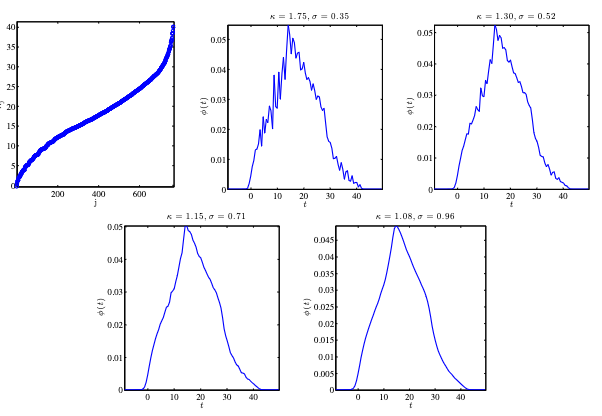
\includegraphics[height=7.5cm]{./Bilder/screenshot.png}
\end{frame}

\begin{frame}
    \frametitle{Regularisierung der Spektraldichte mit Lorentz}
    Die Lorentz-Funktion ist definiert durch
    $$\frac{\eta}{(t - \lambda)^2 + \eta^2} = -\im \left( \frac{1}{t - \lambda + i \eta} \right) \; ,$$
    wobei $\eta$ eine kleine Regularisierungskonstante ist.\\
    Für $\eta \to 0$ nähert sich die Lorentz-Funktion der Dirac-Funktion um den Eigenwert $\lambda$ an\\
    Dies ist z.B. für die Haydock-Methode relevant.
\end{frame}

\begin{frame}
    \frametitle{Die Bedingung der Nicht-Negativität}
    \begin{itemize}
        \item Die Spektraldichte ist als Wahrscheinlichkeitsverteilung nicht-negativ, also
        $$\forall g \in \SR, g \geq 0: \langle \phi, g \rangle \geq 0$$
        \item Einige numerische Annäherungen brechen mit dieser Eigenschaft
        \item Das führt zu großen Fehlern
    \end{itemize}
\end{frame}